%%%%%%%%%%%%%%%%%%%%%%%%%%%%%%%%%%%%%%%%%%%%%%%%%%%%%%%%%%%%%%%%%%%%%%%%%%%%
\chapt[chap:development]{Developing GATE}
\markboth{Developing GATE}{Developing GATE}
%%%%%%%%%%%%%%%%%%%%%%%%%%%%%%%%%%%%%%%%%%%%%%%%%%%%%%%%%%%%%%%%%%%%%%%%%%%%%
\nnormalsize
%%%% qqqqqqqqqqqqqqqqqqqqqqqqq %%%%

%This \chapthing\ describes the protocols to follow and other information for
%those involved in developing GATE.

This \chapthing\ describes ways of getting involved in and contributing to the
GATE project. Sections \ref{sec:development:bugs} and
\ref{sec:development:patches} are good places to start. Sections
\ref{sec:development:creatingplugins} and \ref{sec:development:userguide}
describe protocol and provide information for committers; we cover creating new
plugins and updating this user guide. See Section \ref{sec:development:patches}
for information on becoming a committer.

%%%%%%%%%%%%%%%%%%%%%%%%%%%%%%%%%%%%%%%%%%%%%%%%%%%%%

%%%%%%%%%%%%%%%%%%%%%%%%%%%%%%%%%%%%%%%%%%%%%%%%%%%%%%%%%%%%%%%%%%%%%%%%%%%%%
\sect[sec:development:bugs]{Reporting Bugs and Requesting Features}
%%%%%%%%%%%%%%%%%%%%%%%%%%%%%%%%%%%%%%%%%%%%%%%%%%%%%%%%%%%%%%%%%%%%%%%%%%%%%

The source code and issue trackers for GATE can be found on
\htlink{https://github.com/GateNLP}{GitHub}.  The code is split across many
repositories:
\begin{description}
\item[gate-core] the core GATE Embedded library and GATE Developer GUI.
\item[gate-top] miscellaneous small components including
  \begin{description}
  \item[gate-plugin-base] Maven parent POM shared by all GATE plugins (ours and
    those developed by third parties)
  \item[gate-maven-plugin] Maven plugin used by the base POM to build the
    artifacts required for a JAR to be a GATE plugin
  \item[gate-plugin-test-utils] utilities used in plugin unit tests
  \item[archetypes] to simplify the generation of new plugins
  \end{description}
\item[gate-spring] the helper classes for using GATE in the Spring Framework
  (see section~\ref{sec:api:spring})
\item[gateplugin-*] the standard GATE plugins
\end{description}

Use the GitHub issue tracker for the appropriate repository to report bugs or
submit feature requests -- \verb!gate-core! for bugs in the core library or
which cut across many plugins, or the relevant \verb!gateplugin-! repository
for bugs in a specific plugin.  When reporting bugs, please give as much detail
as possible. Include the GATE version number and build number, the platform on
which you observed the bug, and the version of Java you were using (8u171,
10.0.1, etc.). Include steps to reproduce the problem, and a full stack trace
of any exceptions, including `Caused by \ldots'. You may wish to first check
whether the bug is already fixed in the latest snapshot build (available from
\htlinkplain{https://jenkins.gate.ac.uk}). You may also
request new features.

%%%%%%%%%%%%%%%%%%%%%%%%%%%%%%%%%%%%%%%%%%%%%%%%%%%%%%%%%%%%%%%%%%%%%%%%%%%%%
\sect[sec:development:patches]{Contributing Patches}
%%%%%%%%%%%%%%%%%%%%%%%%%%%%%%%%%%%%%%%%%%%%%%%%%%%%%%%%%%%%%%%%%%%%%%%%%%%%%

Patches may be submitted via the usual GitHub pull request mechanism. Create a
fork of the relevant GitHub repository, commit your changes there, then submit
a pull request.  Note that gate-core is intended to be compatible with Java 8,
so if you regularly develop using a later version of Java it is very important
to compile and test your patches on Java 8.  Patches that use features from a
later version of Java and do not compile and run on Java 8 will not be
accepted.

When you submit a pull request you will be asked to sign a contributor licence
agreement if you do not already have one on file.  This is to ensure that we at
the University of Sheffield have permission to use the code you contribute.

%%%%%%%%%%%%%%%%%%%%%%%%%%%%%%%%%%%%%%%%%%%%%%%%%%%%%%%%%%%%%%%%%%%%%%%%%%%%%
\sect[sec:development:creatingplugins]{Creating New Plugins}
%%%%%%%%%%%%%%%%%%%%%%%%%%%%%%%%%%%%%%%%%%%%%%%%%%%%%%%%%%%%%%%%%%%%%%%%%%%%%

GATE provides a flexible structure where new resources can be plugged in very
easily. There are three types of resources: Language Resource (LR), Processing
Resource (PR) and Visual Resource (VR). In the following subsections we describe
the necessary steps to write new PRs and VRs, and to add plugins to the nightly
build. The guide on writing new LRs will be available soon.

You can quickly create a new plugin project structure using the Maven archetype
described in section~\ref{sec:api:bootstrap}.

%%%%%%%%%%%%%%%%%%%%%%%%%%%%%%%%%%%%%%%%%%%%%%%%%%%%%%%%%%%%%%%%%%%%%%%%%%%%%
\subsect[sec:development:plugin-naming]{What to Call your Plugin}
%%%%%%%%%%%%%%%%%%%%%%%%%%%%%%%%%%%%%%%%%%%%%%%%%%%%%%%%%%%%%%%%%%%%%%%%%%%%%

Plugins in GATE have two types of ``name'', the Maven artifact ID (which is
what you use when adding the plugin to the plugin manager or loading it via the
API) and the \verb!<name>! in the POM file (which is what is displayed in the
plugin manager).  The artifact ID should follow normal Maven conventions and be
named in ``lower-case-with-hyphens'', the human readable name in the POM file
can be anything but conventionally we use the form ``Function: Detail'', for
example ``Language: Arabic'' or ``Tagger: Numbers''.  This naturally groups
similar plugins together in the plugin manager list when it is sorted
alphabetically.  Before naming your plugin, look at the existing plugins and
see where it might group well.

Core GATE plugins use the Maven group ID \verb!uk.ac.gate.plugins!.  If you are
not part of the core GATE development team you should use your own group ID,
typically based on the reversed form of a DNS domain name you control (e.g.
\verb!com.example! if you owned example.com).

%%%%%%%%%%%%%%%%%%%%%%%%%%%%%%%%%%%%%%%%%%%%%%%%%%%%%%%%%%%%%%%%%%%%%%%%%%%%%
\subsect[sec:development:newpr]{Writing a New PR}
%%%%%%%%%%%%%%%%%%%%%%%%%%%%%%%%%%%%%%%%%%%%%%%%%%%%%%%%%%%%%%%%%%%%%%%%%%%%%

\subsubsect{Class Definition}

Below we show a template class definition, which can be used in order to write a
new Processing Resource.

\begin{lstlisting}

package example;

import gate.*;
import gate.creole.*;
import gate.creole.metadata.*;

/**
 * Processing Resource.  The @CreoleResource annotation marks this
 *  class as a GATE Resource, and gives the information GATE needs
 *  to configure the resource appropriately.
 */
@CreoleResource(name = "Example PR",
                comment = "An example processing resource")
public class NewPlugin extends AbstractLanguageAnalyser {

   /* 
    * this method gets called whenever an object of this
    * class is created either from GATE Developer GUI or if 
    * initiated using Factory.createResource() method.
    */
   public Resource init() throws ResourceInstantiationException {
        // here initialize all required variables, and may
        // be throw an exception if the value for any of the
        // mandatory parameters is not provided

        if(this.rulesURL == null)
            throw new ResourceInstantiationException("rules URL null");

        return this;
   }


   /*
    * this method should provide the actual functionality of the PR
    * (from where the main execution begins). This method 
    * gets called when user click on the "RUN" button in the 
    * GATE Developer GUI's application window.     
    */
   public void execute() throws ExecutionException {
        // write code here
   }

   /* this method is called to reinitialize the resource */
   public void reInit() throws ResourceInstantiationException {
       // reinitialization code
   }

   /*
    * There are two types of parameters
    * 1. Init time parameters - values for these parameters need to be 
    * provided at the time of initializing a new resource and these 
    * values are not supposed to be changed.
    * 2. Runtime parameters - values for these parameters are provided  
    * at the time of executing the PR. These are runtime parameters and
    * can be changed before starting the execution 
    * (i.e. before you click on the "RUN" button in GATE Developer)
    * A parameter myParam is specified by a pair of methods getMyParam
    * and setMyParam (with the first letter of the parameter name
    * capitalized in the normal Java Beans style), with the setter
    * annotated with a @CreoleParameter annotation.
    *
    * for example to set a value for outputAnnotationSetName
    */
   String outputAnnotationSetName;

   //getter and setter methods

   /* get<parameter name with first letter Capital>  */
   public String getOutputAnnotationSetName() {
        return outputAnnotationSetName;
   }

   /* The setter method is annotated to tell GATE that it defines an
    * optional runtime parameter.
    */
   @Optional
   @RunTime
   @CreoleParameter(
       comment = "name of the annotationSet used for output")
   public void setOutputAnnotationSetName(String setName) {
        this.outputAnnotationSetName = setName;
   }

   /** Init-time parameter */
   private ResourceReference rulesURL;

   // getter and setter methods
   public ResourceReference getRulesURL() {
      return rulesURL;
   }

   /* This parameter is not annotated @RunTime or @Optional, so it is a
    * required init-time parameter.
    */
   @CreoleParameter(
       comment = "example of an inittime parameter",
       defaultValue = "resources/morph/default.rul")
   public void setRulesURL(ResourceReference rulesURL) {
      this.rulesURL = rulesURL;
   }
}
\end{lstlisting}

Use \verb!ResourceReference! for things like configuration files.  The
\verb!defaultValue! is a path relative to the plugin's
\verb!src/main/resources! folder, but users can use normal URLs to refer to
files outside the plugin's JAR.  Resource files like this should be put into a
\verb!resources! folder (i.e. \verb!src/main/resources/resources!) as GATE
Developer has special support for copying the \verb!resources! folder out of a
plugin to give the user an editable copy of the resource files.

\subsubsect{Context Menu}

Each resource (LR,PR) has some predefined actions associated with
it. These actions appear in a context menu that appears in GATE
Developer when the user right clicks on any of the resources. For
example if the selected resource is a Processing Resource, there will
be at least four actions available in its context menu: 1. Close
2. Hide 3. Rename and 4. Reinitialize. New actions in
addition to the predefined actions can be added by implementing the
\textit{gate.gui.ActionsPublisher} interface in either the LR/PR itself or in
any associated VR. Then the user has to implement the
following method.

\begin{small}\begin{verbatim}

public List getActions() {
     return actions;
}

\end{verbatim}\end{small}

Here the variable \textit{actions} should contain a list of instances of type
\textit{javax.swing.AbstractAction}. A string passed in the constructor of an
AbstractAction object appears in the context menu. Adding a \textit{null} element
adds a separator in the menu.

\subsubsect{Listeners}

There are at least four important listeners which should be implemented in order
to listen to the various relevant events happening in the background. These
include:

\begin{itemize}
\item{CreoleListener}

	Creole-register keeps information about instances of various resources
	and refreshes itself on new additions and deletions. In order to listen
	to these events, a class should implement the
	\textit{gate.event.CreoleListener}. Implementing CreoleListener requires
	users to implement the following methods:

	\begin{itemize}
	\item{public void resourceLoaded(CreoleEvent creoleEvent);}
	\item{public void resourceUnloaded(CreoleEvent creoleEvent);}
	\item{public void resourceRenamed(Resource resource, String oldName, String newName);}
  	\item{public void datastoreOpened(CreoleEvent creoleEvent);}
   	\item{public void datastoreCreated(CreoleEvent creoleEvent);}
   	\item{public void datastoreClosed(CreoleEvent creoleEvent);}
	\end{itemize}

\item{DocumentListener}

	A traditional GATE document contains text and a set of annotationSets.
	To get notified about changes in any of these resources, a class should
	implement the \textit{gate.event.DocumentListener}. This requires users
	to implement the following methods:

	\begin{itemize}
	\item{public void contentEdited(DocumentEvent event);}
	\item{public void annotationSetAdded(DocumentEvent event);}
	\item{public void annotationSetRemoved(DocumentEvent event);}
	\end{itemize}

\item{AnnotationSetListener}

	As the name suggests, AnnotationSet is a set of
	annotations. To listen to the addition and deletion of annotations, a
	class should implement the \textit{gate.event.AnnotationSetListener} and
	therefore the following methods:

	\begin{itemize}
	\item{public void annotationAdded(AnnotationSetEvent event);}
	\item{public void annotationRemoved(AnnotationSetEvent event);}
	\end{itemize}

\item{AnnotationListener}

	Each annotation has a featureMap associated with it, which contains a
	set of feature names and their respective values. To listen to the
	changes in annotation, one needs to implement the
	\textit{gate.event.AnnotationListener} and implement the following
	method:

	\begin{itemize}
	\item{public void annotationUpdated(AnnotationEvent event);}
	\end{itemize}

\end{itemize}


%%%%%%%%%%%%%%%%%%%%%%%%%%%%%%%%%%%%%%%%%%%%%%%%%%%%%%%%%%%%%%%%%%%%%%%%%%%%%
\subsect[sec:development:newvr]{Writing a New VR}
%%%%%%%%%%%%%%%%%%%%%%%%%%%%%%%%%%%%%%%%%%%%%%%%%%%%%%%%%%%%%%%%%%%%%%%%%%%%%

Each resource (PR and LR) can have its own associated visual
resource. When double clicked, the resource's respective visual
resource appears in GATE Developer.  The GATE Developer GUI is divided
into three visible parts (See Figure
\ref{fig:gateguiparts}). One of them contains a tree that shows the loaded
instances of resources. The one below this is used for various purposes - such
as to display document features and that the execution is in progress. This part
of the GUI is referred to as `small'. The third and the largest part of the GUI is
referred to as `large'. One can specify which one of these two should be used for
displaying a new visual resource in the creole.xml.

\begin{figure*}
\center{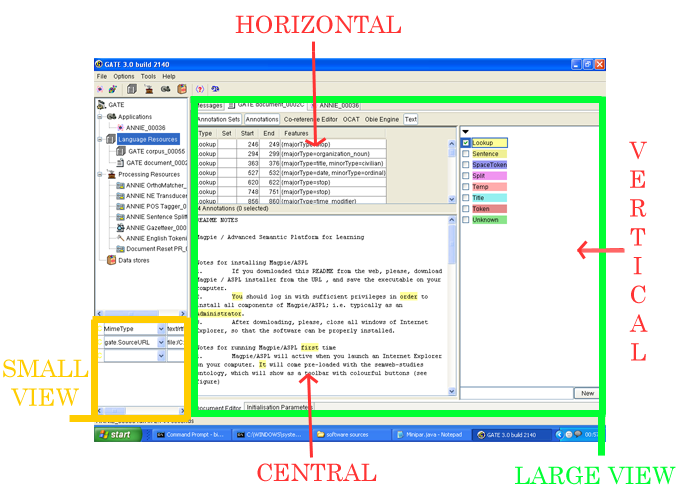
\includegraphics[height=7cm]{gateguiparts.png}} 
\caption{GATE GUI} 
\label{fig:gateguiparts}
\end{figure*}

\subsubsect{Class Definition}

Below we show a template class definition, which can be used in order to write a
new Visual Resource.

\begin{lstlisting}
package example.gui;

import gate.*;
import gate.creole.*;
import gate.creole.metadata.*;

/*
 * An example Visual Resource for the New Plugin
 * Note that here we extends the AbstractVisualResource class.
 * The @CreoleResource annotation associates this VR with the
 * underlying PR type it displays.
 */
@CreoleResource(name = "Visual resource for new plugin",
                guiType = GuiType.LARGE, 
                resourceDisplayed = "example.NewPlugin",
                mainViewer = true)
public class NewPluginVR extends AbstractVisualResource {

     /* 
     * An Init method called when the GUI is initialized for
     * the first time
     */
     public Resource init() {
          // initialize GUI Components
          return this;
     }

     /*
     * Here target is the PR class to which this Visual Resource
     * belongs. This method is called after the init() method.
     */
     public void setTarget(Object target) {
          // check if the target is an instance of what you expected
          // and initialize local data structures if required
     }
}
\end{lstlisting}

Every document has its own document viewer associated with it. It comes with a
single component that shows the text of the original document. GATE provides a
way to attach new GUI plugins to the document viewer. For example AnnotationSet
viewer, AnnotationList viewer and Co-Reference editor. These are the examples of
DocumentViewer plugins shipped as part of the core GATE build. These plugins
can be displayed either on the right or on top of the document viewer. They can also
replace the text viewer in the center (See figure \ref{fig:gateguiparts}). A
separate button is added at the top of the document viewer which can be pressed
to display the GUI plugin.

Below we show a template class definition, which can be used to develop a new
DocumentViewer plugin.

\begin{lstlisting}

/*
 * Note that the class needs to extends the AbstractDocumentView class
 */
@CreoleResource
public class DocumentViewerPlugin extends AbstractDocumentView {

     /* Implementers should override this method and use it for
      * populating the GUI.
      */
          public void initGUI() {
               // write code to initialize GUI   
          }

          /* Returns the type of this view */
          public int getType() {
               // it can be any of the following constants 
               // from the gate.gui.docview.DocumentView
               // CENTRAL, VERTICAL, HORIZONTAL
          }

          /* Returns the actual UI component this view represents. */
          public Component getGUI() {
               // return the top level GUI component 
          }

          /* This method called whenever view becomes active.*/
          public void registerHooks() {
               // register listeners
          }

          /* This method called whenever view becomes inactive. */
          public void unregisterHooks() {
               // do nothing
          }
}
\end{lstlisting}

%%%%%%%%%%%%%%%%%%%%%%%%%%%%%%%%%%%%%%%%%%%%%%%%%%%%%%%%%%%%%%%%%%%%%%%%%%%%%
\subsect[sec:development:readymade]{Writing a `Ready Made' Application}
%%%%%%%%%%%%%%%%%%%%%%%%%%%%%%%%%%%%%%%%%%%%%%%%%%%%%%%%%%%%%%%%%%%%%%%%%%%%%

Often a CREOLE plugin may contain an example application to showcase the
PRs it contains. These `ready made' applications can be made easily available
through GATE Developer by creating a simple {\tt PackagedController} subclass.
In essence such a subclass simply references a saved application and provides
details that can be used to create a menu item to load the application.

The following example shows how the example application in the
{\tt tagger-measurements} plugin is added to the menus in GATE Developer.

\begin{lstlisting}
@CreoleResource(name = "ANNIE+Measurements",
   icon = "measurements", autoinstances = @AutoInstance(parameters = {
   @AutoInstanceParam(name="pipelineURL",
                      value="resources/annie-measurements.xgapp"),
   @AutoInstanceParam(name="menu", value="ANNIE")}))
public class ANNIEMeasurements extends PackagedController {

}
\end{lstlisting}

The menu parameter is used to specify the folder structure in which the menu
item will be placed. Typically its value will just be a single menu name, but
it can be a semicolon-separated list of names, which will map to a series of
sub-menus.  For example \verb!"Languages;German"! would create a ``Languages''
menu with a ``German'' sub-menu, which in turn would contain the menu item
for this application.


%%%%%%%%%%%%%%%%%%%%%%%%%%%%%%%%%%%%%%%%%%%%%%%%%%%%%%%%%%%%%%%%%%%%%%%%%%%%%
\subsect[sec:development:disributingplugins]{Distributing Your New Plugins}
%%%%%%%%%%%%%%%%%%%%%%%%%%%%%%%%%%%%%%%%%%%%%%%%%%%%%%%%%%%%%%%%%%%%%%%%%%%%%

Since GATE 8.5 plugins are distributed via the normal Maven repository
mechanism.  Release versions of most core plugins are in the Central
Repository and snapshot versions are released via our own Maven repository at
\htlinkplain{http://repo.gate.ac.uk/content/groups/public}, along with releases
of a few plugins whose dependencies are not in Central.

There are several routes by which you can release your own plugins into the
Central Repository, the simplest is to use the Sonatype
\htlink{http://central.sonatype.org}{OSSRH} system (which is how we release
\verb!gate-core! and the standard plugins).

For snapshots you can host your own Maven repository, or use the OSSRH snapshot
repository.  In order to use plugins from a repository other than Central or
the GATE team repository mentioned above, you must tell Maven where to find it
by creating a file called \verb!settings.xml! in the \verb!.m2! folder under
your home directory -- GATE will respect any repositories you have configured
in your Maven settings.
\begin{lstlisting}[lang=XML]
<settings xmlns="http://maven.apache.org/SETTINGS/1.0.0"
  xmlns:xsi="http://www.w3.org/2001/XMLSchema-instance"
  xsi:schemaLocation="http://maven.apache.org/SETTINGS/1.0.0
                      http://maven.apache.org/xsd/settings-1.0.0.xsd">

  <profiles>
    <profile>
      <id>my-custom-repo</id>
      <repositories>
        <repository>
            <id>my-repo</id>
            <name>My Personal Repo</name>
            <url>http://repo.example.com/</url>
            <layout>default</layout>
            <releases><enabled>true</enabled></releases>
            <snapshots><enabled>true</enabled></snapshots>
          </repository>
      </repositories>
    </profile>
  </profiles>

  <activeProfiles>
    <activeProfile>my-custom-repo</activeProfile>
  </activeProfiles>
</settings>
\end{lstlisting}

%%%%%%%%%%%%%%%%%%%%%%%%%%%%%%%%%%%%%%%%%%%%%%%%%%%%%%%%%%%%%%%%%%%%%%%%%%%%%
\sect[sec:development:defaultplugins]{Adding your plugin to the default list}
%%%%%%%%%%%%%%%%%%%%%%%%%%%%%%%%%%%%%%%%%%%%%%%%%%%%%%%%%%%%%%%%%%%%%%%%%%%%%

The GATE plugin manager has a list of ``default'' plugins that are
automatically listed in the manager whenever GATE Developer is started.  This
list is itself maintained in another GitHub repository
\htlinkplain{https://github.com/GateNLP/gate-metadata}, with a separate file
for each version of GATE.  If you have developed and released a plugin that you
believe is of wider interest to the GATE user community you can request that it
be added to the default list.  This is done through the normal GitHub pull
request mechanism -- fork the \verb!gate-metadata! repository and commit your
change to all the versioned \verb!plugins-NNN.tsv! files for versions of GATE
with which your plugin is compatible, then submit a pull request asking us to
merge your change into the master list.

The same procedure applies when you release an updated version of your plugin
-- update your forked copy of the TSV files and submit another pull request.

%%%%%%%%%%%%%%%%%%%%%%%%%%%%%%%%%%%%%%%%%%%%%%%%%%%%%%%%%%%%%%%%%%%%%%%%%%%%%
\sect[sec:development:userguide]{Updating this User Guide}
%%%%%%%%%%%%%%%%%%%%%%%%%%%%%%%%%%%%%%%%%%%%%%%%%%%%%%%%%%%%%%%%%%%%%%%%%%%%%

The GATE User Guide is maintained on GitHub at
\htlinkplain{https://github.com/GateNLP/userguide}.  If you are a developer at
Sheffield you do not need to check out
the userguide explicitly, as it will appear under the \texttt{tao} directory
when you check out \texttt{sale}.

The user guide is written in \LaTeX\ and translated to PDF using
\texttt{pdflatex} and to HTML using \texttt{tex4ht}.  The main file that ties
it all together is \verb|tao_main.tex|, which defines the various macros used
in the rest of the guide and \verb|\input|s the other \texttt{.tex} files, one
per chapter.

%%%%%%%%%%%%%%%%%%%%%%%%%%%%%%%%%%%%%%%%%%%%%%%%%%%%%%%%%%%%%%%%%%%%%%%%%%%%%
\subsect[sec:development:ug-build]{Building the User Guide}
%%%%%%%%%%%%%%%%%%%%%%%%%%%%%%%%%%%%%%%%%%%%%%%%%%%%%%%%%%%%%%%%%%%%%%%%%%%%%

You will need:
\begin{itemize}
\item
A standard POSIX shell environment including GNU Make.  On Windows this
generally means \htlink{http://www.cygwin.com}{Cygwin}, on Mac OS X the XCode
developer tools and on Unix the relevant packages from your distribution.
\item
A copy of the userguide sources (see above).
\item
A \LaTeX\ installation, including pdflatex if you want to build the PDF
version, and tex4ht if you want to build the HTML.  MiKTeX should work for
Windows, texlive (available in \htlink{http://www.macports.org}{MacPorts}) for
Mac OS X, or your choice of package for Unix.
\item
The BibTeX database \texttt{big.bib}.  It must be located in the directory
\textbf{above} where you have checked out the userguide, i.e. if the guide
sources are in \verb|/home/bob/github/userguide| then \texttt{big.bib} needs to go
in \verb|/home/bib/github|.  Sheffield developers will find that it is already in
the right place, under \texttt{sale}, others will need to download it from
\htlinkplain{http://gate.ac.uk/sale/big.bib}.
\item
The file \htlinkplain{http://gate.ac.uk/sale/utils.tex}.
\item
A bit of luck.
\end{itemize}

Once these are all assembled it \emph{should} be a case of running
\texttt{make} to perform the actual build.  To build the PDF do
\texttt{make tao.pdf}, for the one page HTML do \texttt{make index.html} and
for the several pages HTML do \texttt{make split.html}.

The PDF build generally works without problems, but the HTML build is known to
hang on some machines for no apparent reason.  If this happens to you try again
on a different machine.

%%%%%%%%%%%%%%%%%%%%%%%%%%%%%%%%%%%%%%%%%%%%%%%%%%%%%%%%%%%%%%%%%%%%%%%%%%%%%
\subsect[sec:development:ug-changes]{Making Changes to the User Guide}
%%%%%%%%%%%%%%%%%%%%%%%%%%%%%%%%%%%%%%%%%%%%%%%%%%%%%%%%%%%%%%%%%%%%%%%%%%%%%

To make changes to the guide simply edit the relevant \texttt{.tex} files, make
sure the guide still builds (at least the PDF version), and check in your
changes \textbf{to the source files only}.  Please do not check in your own
built copy of the guide, the official user guide builds are produced by a
Jenkins continuous integration server in Sheffield.

For non-Sheffield developers we welcome documentation patches through the
normal GitHub pull request mechanism.

If you add a section or subsection you should use the \verb|\sect| or
\verb|\subsect| commands rather than the normal LaTeX \verb|\section| or
\verb|\subsection|.  These shorthand commands take an optional first parameter,
which is the label to use for the section and should follow the pattern of
existing labels.  The label is also set as an anchor in the HTML version of
the guide.  For example a new section for the `Fish' plugin would go in
\verb|misc-creole.tex| with a heading of:
\begin{small}\begin{verbatim}
\sect[sec:misc-creole:fish]{The Fish Plugin}
\end{verbatim}\end{small}
and would have the persistent URL
\verb|http://gate.ac.uk/userguide/sec:misc-creole:fish|.

If your changes are to document a bug fix or a new (or removed) feature then you
should also add an entry to the change log in \verb|recent-changes.tex|. You
should include a reference to the full documentation for your change, in the same
way as the existing changelog entries do. You should find yourself adding to the
changelog every time except where you are just tidying up or rewording existing
documentation. Unlike in the other source files, if you add a section or
subsection you should use the \verb|\rcSect| or \verb|\rcSubsect|. Recent
changes appear both in the introduction and the appendix, so these commands
enable nesting to be done appropriately.

Section/subsection labels should comprise `sec' followed by the chapter label and
a descriptive section identifier, each colon-separated. New chapter labels should
begin `chap:'.

Try to avoid changing chapter/section/subsection labels where possible, as this
may break links to the section. If you need to change a label, add it in the
file `sections.map'. Entries in this file are formatted one per line, with the
old section label followed by a tab followed by the new section label.

The quote marks used should be ` and '.

Titles should be in title case (capitalise the first word, nouns, pronouns,
verbs, adverbs and adjectives but not articles, conjunctions or prepositions).
When referring to a numbered chapter, section, subsection, figure or table,
capitalise it, e.g. `Section 3.1'. When merely using the words chapter, section,
subsection, figure or table, e.g. `the next chapter', do not capitalise them.
Proper nouns should be capitalised (`Java', `Groovy'), as should strings where
the capitalisation is significant, but not terms like `annotation set' or
`document'.

The user guide is rebuilt automatically whenever changes are checked in, so
your change should appear in the online version of the guide within 20 or 30
minutes.
